\documentclass[14pt]{extarticle}
\usepackage[utf8]{inputenc}
\usepackage{ngerman}
\usepackage{array}
\usepackage{amsmath}
\title{Bericht Todesstern U1}
\author{Charline Waldrich, Robert Ullmann, Julian Dobrot}
\date{30. Oktober 2015}

\begin{document}

\maketitle
\pagebreak
\tableofcontents


\section{Aufgabenstellung}

\subsection{ImageViewer}
Der ImageViewer ist ein Programm mit dem eine Bilddatei von der Festplatte ausgewählt werden kann und dieses in der GUI angezeigt wird. 
\subsection{ImageSaver}
Der ImageSaver ist ein Programm walches ein Bild erzeugt, dass so groß ist wie das Fenster.
Das Bild ist Schwarz und beinhaltet einen diagonalen roten Strich. Über eine Menüzeile kann das Bild in den Formaten PNG und JPG gespeichert werden.
\subsection{Matrizen- und Vectorenbibliothek}
Die Matritzen- und Vektorenbibliothek beinhaltet die folgenden fünf Klassen mit ihren Methoden um Operationen 
zur berechnung mit Matrix- und Vectorobjekten durchführen zu können:

\begin{itemize}
\item Eine Main, um die Testfälle aus der Aufgabenstellung durchzuführen.
\item Point3
\item Mat3x3
\item Vector3 
\item Normal3
\end{itemize}


\section{Lösungsstrategien}
\subsection{ImageViewer}
Der ImageViewer öffnet beim Starten einen Dialog um eine Bilddatei im PNG oder JPG- Format auszuwählen. Das ausgewählte Bild wird in einem Fenster, passend zur Größe, angezeigt.
\subsection{ImageSaver}
Der ImageSaver nutzt als Grundlage die JavaFX Applikation. Ich habe mich für die VBox als Grundlage des Fensters entscheiden da diese alle hinzugefügten Elemente automatisch untereinander anordnet. Um ein Bild Pixel für Pixel zu erzeugen, braucht es ein WritableImage Objekt welches der ImageView übergeben wird, um es darzustellen und abzuspeichern. 
\newline
Das erzeugte Bild muss in ein BufferedImage umgewandelt werden um die Speicherung zu ermöglichen. Als PNG Datei kann es ohne große Umwege umgewandelt werden, doch da eine JPG Datei einen Alpha-Kanal besitzt ist diese Art der Speicherung erst nach dem erstellen eines weiteren BufferedImage mit Byte Basiertem Index, welches danach in eine 2D Grafik umgewandelt werden muss, möglich.  

\subsection{Matrizen- und Vektorenbibliothek}
Die Klassen wurden nach den Klassendiagrammen angelegt und erfüllen die im Aufgabentext beschriebenen mathematischen Operationen. Die im vorherigen Semester erlernten mathematischen Fähigkeiten  wurden angewendet um die Problemstellungen zu realisieren und programmiertechnisch umzusetzen. Zur Lösung der reflectedOn Methode wurde die Mathematik recherchiert und umgesetzt.

\section{Implementierungen}
\subsection{ImageViewer}
Der ImageViewer besteht aus zwei Methoden. Die erste Methode ist die Java-FX \textbf{start}-Methode, welche das Layout beinhaltet. Dieses besteht aus einer BorderPane und darin enthalten eine ImageView, welche das Bild anzeigt. \\
Die zweite Methode ist die \textbf{openFileDialog}-Methode. Diese Methode dient der Auswahl des Bildes und gibt das ausgewählte File zurück an die start-Methode.
\subsection{ImageSaver}
Die ImageSaver Klasse besteht aus zwei öffentlichen Methoden, start und main. 
Hinzu kommen vier private Methoden. Die initializeMenu Methode zum Einrichten der Menüleiste, welche in der Startmethode aufgerufen wird, zwei Methoden zum Erstellen des Bildes und eine weitere zum Abspeichern dessen. 
\newline
Die drawPicture Methode wird in der Start Methode aufgerufen sobald sich die Höhe oder Breite des Fensters ändert. Diese wiederum ruft in einer verschachtelten for-Schleife die getColor Methode auf, welche für jeden Bildpixel mit den übergebenen Koordinaten x und y, die Farbgebung bestimmt. 
\newline
In der saveFile Methode wird der Speicherdialog Initialisiert und die Möglichkeit das Pixelbild als JPG oder PNG Datei zu speichern wird gegeben. 
\newline
Eine Verknüpfung der beiden Klassen ImageSaver und ImageViewer wäre eine sinnvolle Implementierung, denn durch hinzufügen einiger Menüpunkte könnte man so dem User die Möglichkeit bieten sich zwischen dem erstellen eines pixelbasiertem, oder dem Anzeigen eines bereits existierendem Bildes zu entscheiden. 

\subsection{Matrizen- und Vektorenbibliothek}
\textbf{Point3:} Ein Punkt im dreidimensionalem Raum mit seinen x,y,z Werten. Die Klasse stellt Methoden bereit um einen Punkt mit anderen Objekten aus der Bibliothek zu subtrahieren und zu addieren.
\\\textbf{Mat3x3:} Im Konstruktor dieser Klasse sollen die neun Elemente einer 3x3 Matrix übergeben werden und die Determinante dieser Matrix wird bei der Initialisierung berechnet. Die Klasse enthält verschiedene Methoden um Operationen mit der übergebenen Matrix durchzuführen und diese zu verändern. 
\\\textbf{Normal3:} Eine Normale auf einer Oberfläche. Die x,y,z Werte der Normalen werden bei ihrer Initialisierung als unveränderliche Attribute übergeben. Des weiteren enthält die Klasse Methoden für Operationen zur Berechnung von Multiplikationen mit double Werten, die Addition mit anderen Normal3 Objekten und dem Kreuzprodukt mit Vektoren.
\\\textbf{Vector3:} Diese Klasse stellt einen dreidimensionalen Vektor dar und ermöglicht mit ihren Methoden verschiedene Operationen.


\section{Besondere Probleme oder Schwierigkeiten bei der Bearbeitung}
\subsection{ImageViewer}
Bei der Implementierung des ImageViewers kam es zu keinen besonderen Problemen oder Schwierigkeiten.
\subsection{ImageSaver}
Damit der ImageSaver, jedes Mal wenn der Nutzer die Größe des Fensters verstellt, ein neues Pixelbild mit passender Größe kreiert, hätte ich gern mit einem PropertyBinding gearbeitet. 
Leider bietet weder die ImageViewer noch die WritableImage Klasse ein solches an. Daher habe ich die Klasse so geschrieben, dass die DrawPicture Methode (dank eines Listeners) jedes Mal aufs Neue aufgerufen wird, wenn sich Höhe oder Breite des Fensters ändern. 
\newline
Damit nicht mehrere Bilder dem Fenster hinzugefügt werden, wird zu Anfang des Methodenaufrufs die ImageView stets von der Bilduntergrundfläche (VBox root) gelöscht und nach erstellen des neuen Bildes wieder hinzugefügt. 
\subsection{Matrizen- und Vektorenbibliothek}
Für die reflectedOn Methode wurde die Formel 
\begin{math} R=2(N*L)N-L \end{math}
angewendet.  Wobei R der reflektierte Vektor ist, N die Normale an der reflektiert wird und L ein normalisierter Vektor der in Richtung der Lichtquelle zeigt, dies ist das über den Parameter der Methode übergebene Normal3 Objekt. Die Schwierigkeit in der Umsetzung der Mathematik in den Programmcode bestand darin, dass die Formel umgestellt werden musste. So wird in der Methode erst die übergebene Normale mit -1 multipliziert, was den letzten Teil der Formel repräsentiert. 

\section{Zeitbedarf}
\begin{center}
\begin{tabular}{cr}
ImageViewer	  \	&80 min	\\
ImageSaver 	\	&240 min	\\
Bibliotheken \	&240 min	\\
Bericht  \		&180 min	 \\
	\hline
	&740 min
\end{tabular}
\end{center}

\section{Quellen}
https://asalga.wordpress.com/2012/09/23/understanding-vector-reflection-visually/

\section*{2. Abgabe}

\section{Ray}
Die ,,Ray'' Klasse initialisiert einen Strahl mit gegebenem Ausgangspunkt und Richtungsvektor. Sie implementiert zwei Methoden namens ,,at'' und ,,tOf''. Außerdem wurden die von der Oberklasse Object geerbten Methoden hashCode und eqals so überschrieben, dass sie zum Testen nützlich sind.\\
Der Strahl (Ray) kann mit der Methode ,,at'' den Punkt berechnen, welchen er trifft wenn er die als Parameter übergebenen Länge ,,t'' (als double Wert), den Richtungsvektor ''entlang geht''. Hierfür wird die eine einfache Rechnung angewandt. 
$$ Punt P = Ausgangspunkt O + Länge t \times Richtungsvektor d $$
In der Methode ,,tOf'' wird diese Rechnung umgedreht. Ein gesuchter Punkt wird als Parameter übergeben und berechnet dann den Faktor ,,t'' (als double Wert) welcher mit dem Richtungsvektor multipliziert werden müsste um zu gesuchtem Punkt zu gelangen. \\

\section{Hit}
Das Hit Objekt bekommt einen double Wert ,,t'', einen Strahl ,,ray'' und eine geometrische Figur übergeben und zugewiesen. Außerdem werden in der Klasse die von der Oberklasse Object vererbten Methoden ,,toString'', ,,hashCode'' und ,,equals'' überschrieben.

\section{World}
Die Klasse ,,World'' initialisiert ein Fenster mit übergebener Hintergrundfarbe. Diese soll zukünftig vom Nutzer ausgewählt werden. Sie beinhaltet eine Array Liste in welcher nur Objekte des Typs ,,Geometry'' gespeichert werden können.\\ 
Des weiteren gibt es eine Methode namens ,,hit'' welche einen Strahl (Ray) übergeben bekommt und eine Farbe vom Typ Color zurück gibt. Zunächst wird ein Hit Objekt ,,hit0'' der mit dem null-Wert initialisiert. \\
In der for-Schleife wird für jedes Objekt in der Liste ein weiteres Hit Objekt mit dem übergebenen Strahl gespeichert. Hält das ,,hit1'' Objekt einen Wert welcher ungleich null ist und liegt vor den anderen Objekten (hat also ein kleineren ,,t''-Wert, als die Objekte welche davor in hit0 gespeichert wurden), so wird der außen liegenden Variable ,,hit0'' dieses Hit Objekt zugewiesen. Sollte nach dem Durchgang der kompletten Schleife der Wert von ,,hit0'' immer noch null sein, so wird die Hintergrundfarbe der Welt zurück gegeben. Wenn nicht so wird immer die Farbe des am nächstliegendsten Objekt zurück gegeben. 

\section{Geometry}
\subsection{Plane}
Die Klasse Plane beschreibt eine Ebene. Diese wird genau definiert durch die übergebenen Parameter; einen auf der Ebene liegenden Punkt, einem Normalen-Vektor welcher die Ausrichtung (bzw. Neigung) der Ebene definiert, und einem Color Objekt welche die Farbe der Ebene hält. \\
Die von der Oberklasse Object geerbten Methoden ,,toString'', ,,hashCode'' und ,,equals'' wurden sinnvoll überschrieben.\\
Des weiteren wird die Methode ,,hit'' von der abstrakten Oberklasse Geometry vererbt und auf die Ebene angepasst. Diese bekommt einen Strahl übergeben welcher nicht null sein darf und gibt ein Hit Objekt zurück. Danach wird zunächst getestet ob das Skalarprodukt des Strahls und des Normalenvektor gleich Null ist. Ist dies der Fall sind Ebene und Strahl paralell und ,,null'' wird zurück gegeben. \\
Ist dies nicht der Fall, wird für den Strahl und die Ebene die Entfernung berechnet. \\
Ist diese kleiner Null bedeutet das, dass das Objekt vor dem Ortsvektor des Strahls (und somit vor unserer Bildschirmfläche) liegt und es wird wieder ein ,,null'' Objekt zurück geliefert. \\
Ist der berechnete double-Wert größer 0 wird ein Hit Objekt mit dem berechneten ,,t''-Wert, dem der Methode übergebenen Ray ,,r'' und der im Konstruktor zugewiesenen Farbe zurück gegeben (siehe Abb. \ref{Ebene}).\\
Außerdem wird in unserer Color Klasse der RGB-Wert berechnet, welcher für das färben des writableImage Objektes nicht brauchbar ist. Da der pixelWriter nur Color Objet aus dem javaFX Paket erkennt, müssen die einzeln berechneten Werte an ein neues Color Objekt dessen übergeben werden.
\begin{figure}[ht]
\begin{center}
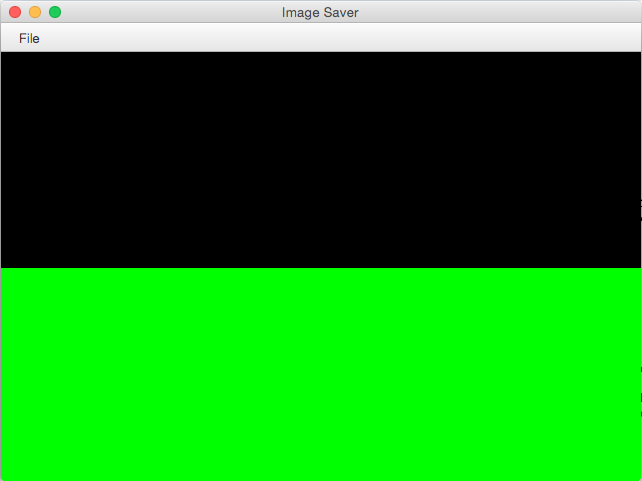
\includegraphics[width=5cm, height=8cm]{TestCase1.png}
\caption{Ebene aus Perspektivischer Kamera}
\label{Ebene}
\end{center}
\end{figure}

\subsection{Sphere}
Die Klasse Sphere representiert die Geometrie einer Kugel
\subsection{AxisAlignedBox}
Diese Klasse ermöglicht es Box Objekte zu erzeugen
\section{Besondere Probleme oder Schwierigkeiten bei der Bearbeitung}
\subsection{Tests}
In der ImageSaver Klasse musste die ,,getColor''-Methode angepasst werden. Diese benutzt unsere persönliche Color Klasse und berechnet für jeden einzelnen Pixel dank der ,,hit'' Methode der Welt, ob das erzeugte Objekt von dem Strahl der erzeugten Klasse getroffen wird. Da in der Bildverarbeitung der Ursprung des Koordinatensystems oben links und in der Mathematik unten links liegt, musste bei der Berechnung aufgepasst werden, dass der ,,rayFor'' Methode welche von der ,,camera'' aufgerufen wird. nicht die oben liegende Y-Koordinate übergeben wird, sondern dem quasi spiegelverkehrtem Pixel unten. 

-> hier kannst du rein schreiben was bei der Camera Klasse das Problem war und wie es schön das ganze Projekt kaputt gemacht hat ;) 

\end{document}